\subsection{Implementation of Newton's Method}
When implementing Newton's Method both the gradient and the Hessian of the performance function \eqref{performanceFunction} are needed.
%
\begin{flalign}
	\frac{\partial  }{\partial \vec{\theta}} P(\vec{\theta}) &= \vec{G}(\vec{\theta}) = \frac{\partial}{\partial \vec{\theta}} \left( \frac{1}{2N}\sum_{k = 1}^{N} \left(\vec{y}(kT) - \vec{y_m}(kT, \vec{\theta})\right)^2 \right) &
\end{flalign}
\begin{flalign}
  \eq{\vec{G}(\vec{\theta})} {- \frac{1}{N}\sum_{k = 1}^{N} \left((\vec{y}(kT) - \vec{y_m}(kT, \vec{\theta})) \ \frac{\partial  }{\partial \vec{\theta}} \ \vec{y_m}(kT, \vec{\theta}) \right) } &
\label{gradientOfPerformanceFunction}
\end{flalign}
%\begin{flalign}
%	\frac{\partial \vec{P}(\vec{\theta}) }{\partial \vec{\theta}} &= G(\vec{\theta}) = \frac{\partial}{\partial \vec{\theta}} \left( \frac{1}{2N}\sum_{k = 1}^{N} \left(\vec{y}(kT) - \vec{y_m}(kT, \vec{\theta})\right)^2 \right) &\\
%  \eq{\vec{G}(\vec{\theta})} {- \frac{1}{N}\sum_{k = 1}^{N} \left((\vec{y}(kT) - \vec{y_m}(kT, \vec{\theta})) \ \frac{\partial  \vec{y_m}(kT, \vec{\theta})}{\partial \vec{\theta}} \right) } &
%\label{gradientOfPerformanceFunction}
%\end{flalign}

Since the Matlab implementation uses a Simulink model the problematic part of \eqref{gradientOfPerformanceFunction} is the derivative of the model with respect to the model parameters, \si{\frac{\partial  }{\partial \vec{\theta}}\ \vec{y_m}(kT, \vec{\theta})}. To solve this problem a numerical differentiation of the model is applied as shown in \autoref{AlgorithmForNummericalDiff}.

\begin{lstlisting}[ language = Matlab,
                    caption  = {Algorithm for numerical differentiation of the simulated model},
                    label    = AlgorithmForNummericalDiff ]

  %small deviation from parameters, J_f and B_f, is set
  p = 0.001;
  
  %calculating the deviation
  deltaJ_f = p*J_f; deltaB_f = p*B_f;
  
  %saving the old parameters:
  J_f_old = J_f; B_f_old = B_f;
  
  %setting deviating parameters ready for simulation
  J_f = deltaJ_f;
  
  %running the simulation again, now with deviation in J_f
  sim('CubliParameterEstimation.slx');
  
  %storring the result of the simulation
  deltaYmJf = simOut;
  
  %setting deviating parameters ready for simulation
  B_f = deltaB_f; J_f = J_f_old; %<--restoring J_f
  
  %running the simulation again, now with deviation in B_f
  sim('CubliParameterEstimation.slx');
  
  %storring the result of the simulation
  deltaYmBf = simOut;
  
  %restoring the parameters to their original value
  B_f = B_f_old;
  
  %calculating the derivatives of the model
  YmDiffBf = ( deltaYmBf - Ym )/ p;
  YmDiffJf = ( deltaYmJf - Ym )/ p;
\end{lstlisting}

Now that the model partial derivatives are found, all parts of the gradient, as represented in \eqref{gradientOfPerformanceFunction}, are known. The Hessian is also needed and can be represented as,
%
\begin{flalign}
	\vec{H}(\vec{\theta}) &= \frac{\partial^2 }{\partial \vec{\theta}^2}\  P(\vec{\theta}) = \frac{\partial }{\partial \vec{\theta}} \ \vec{G}(\vec{\theta}) &
\end{flalign}
%
which leads to the following:
\begin{flalign}
	\vec{H}(\vec{\theta}) &= \frac{1}{N}\sum_{k = 1}^{N} \left(     \frac{\partial  }{\partial \vec{\theta}} \ \vec{y_m}(kT, \vec{\theta}) \left(\frac{\partial }{\partial \vec{\theta}} \ \vec{y_m}(kT, \vec{\theta}) \right)^T  	  - \left(\frac{\partial^2  }{\partial \vec{\theta}^2} \ \vec{y_m}(kT, \vec{\theta}) \right) (\vec{y}(kT) - \vec{y_m}(kT, \vec{\theta}))  \right) &
\label{hessianOfPerformanceFunction}
\end{flalign}
%\begin{flalign}
%	\vec{H}(\vec{\theta}) &= \frac{1}{N}\sum_{k = 1}^{N} \left(   \left\Vert \frac{\partial  \vec{y_m}(kT, \vec{\theta})}{\partial \vec{\theta}} \right\Vert_2^2  	  - \left(\frac{\partial^2 \vec{y_m}(kT, \vec{\theta}) }{\partial^2 \vec{\theta}^2}\right) (\vec{y}(kT) - \vec{y_m}(kT, \vec{\theta}))  \right) &
%\label{hessianOfPerformanceFunction}
%\end{flalign}
%\begin{flalign}
%	\vec{H}(\vec{\theta}) &= \frac{1}{N}\sum_{k = 1}^{N} \left(   \frac{\partial  \vec{y_m}(kT, \vec{\theta})}{\partial \vec{\theta}} \left(\frac{\partial \vec{y_m}(kT, \vec{\theta})}{\partial \vec{\theta}} \right)^T  	  - \left(\frac{\partial^2 \vec{y_m}(kT, \vec{\theta}) }{\partial^2 \vec{\theta}^2}\right) (\vec{y}(kT) - \vec{y_m}(kT, \vec{\theta}))  \right) &
%\label{hessianOfPerformanceFunction}
%\end{flalign}
%
To avoid the second derivative of the performance function in \eqref{hessianOfPerformanceFunction}, the Hessian can be approximated simply by removing this last term.
\begin{flalign}
	\vec{\widetilde{H}}(\vec{\theta}) &\triangleq \frac{1}{N}\sum_{k = 1}^{N} \frac{\partial  }{\partial \vec{\theta}} \ \vec{y_m}(kT, \vec{\theta}) \left(\frac{\partial }{\partial \vec{\theta}} \ \vec{y_m}(kT, \vec{\theta}) \right)^T &
\label{hessianApproxOfPerformanceFunction}
\end{flalign}
%\begin{flalign}
%	\vec{\widetilde{H}}(\vec{\theta}) &\triangleq \frac{1}{N}\sum_{k = 1}^{N} \ \left\Vert  \frac{\partial  \vec{y_m}(kT, \vec{\theta})}{\partial \vec{\theta}} \right\Vert_2^2 &
%\label{hessianApproxOfPerformanceFunction}
%\end{flalign}
%\begin{flalign}
%	\vec{\widetilde{H}}(\vec{\theta}) &\triangleq \frac{1}{N}\sum_{k = 1}^{N} \left(   \frac{\partial  \vec{y_m}(kT, \vec{\theta})}{\partial \vec{\theta}} \left(\frac{\partial \vec{y_m}(kT, \vec{\theta})}{\partial \vec{\theta}} \right)^T \right) &
%\label{hessianApproxOfPerformanceFunction}
%\end{flalign}
%
This approximation assumes that the model is only linearly dependent on the parameters, \si{\vec{\theta}}. As the error term, \si{(\vec{y}(kT) - \vec{y_m}(kT, \vec{\theta}))}, approaches zero the approximation becomes increasingly accurate.

Running the implementation of Newton's method approximates the model parameters to \si{J_F = } and \si{B_F = }, while giving a normed root mean square error of \si{31,71 \%} as seen on \figref{ParameterEstimationNewtonCubli}. %The normed RMS error is a way to determine the goodness of the fit.

\begin{figure}[H] 
	\centering
	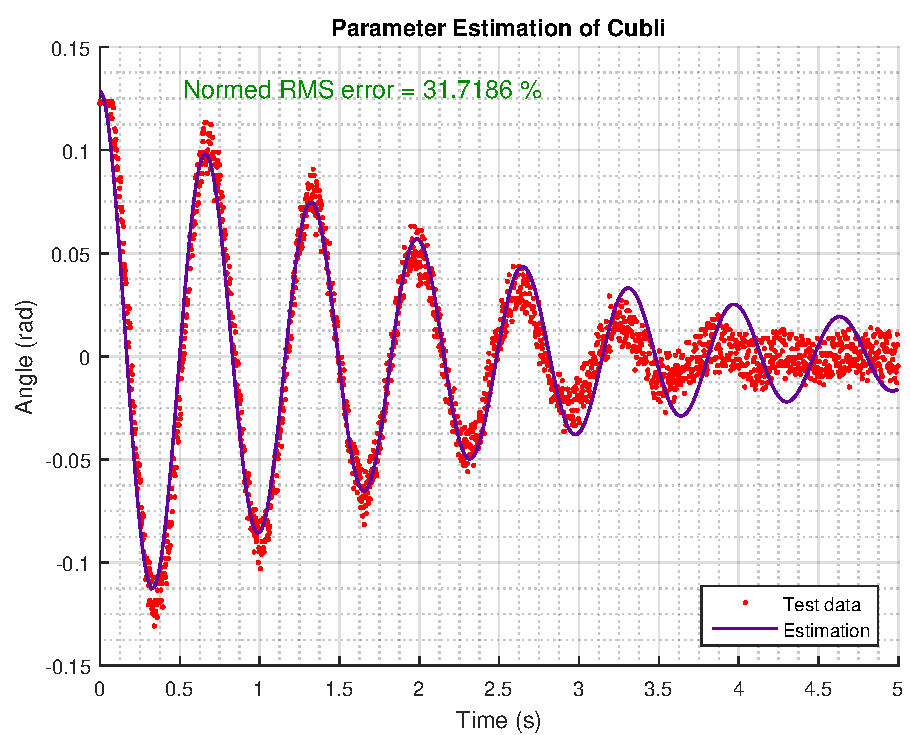
\includegraphics[width=.8\textwidth]{figures/ParameterEstimationNewtonCubli}
	\caption{The result of implementation of Newton's method}
	\label{ParameterEstimationNewtonCubli}
\end{figure}